% Template for ICIP-2015 paper; to be used with:
%          spconf.sty  - ICASSP/ICIP LaTeX style file, and
%          IEEEbib.bst - IEEE bibliography style file. cambio para probar adsfasfasfasfsf
% --------------------------------------------------------------------------
\documentclass[spanish,twocolumn]{article}
\usepackage{spconf,amsmath,graphicx}
\usepackage{mathptmx}
\usepackage{mathtools}
\usepackage{amsmath}
\usepackage{mathrsfs}
\usepackage{amssymb}
\usepackage{amsfonts}
\usepackage[utf8]{inputenc}
\usepackage{babel}
\usepackage{color}
\usepackage[Algoritmo]{algorithm}
\usepackage{algpseudocode}
\usepackage{multicol}
\usepackage{caption,setspace}
\usepackage{subfig}

\algrenewcommand\algorithmicif{\textbf{si}}
\algrenewcommand\algorithmicend{\textbf{fin}}
\algrenewcommand\algorithmicfor{\textbf{para}}
\algrenewcommand\algorithmicdo{\textbf{hacer}}
\algrenewcommand\algorithmicwhile{\textbf{mientras}}
\algrenewcommand{\algorithmicrequire}{\textbf{Entrada:}}
\algrenewcommand{\algorithmicensure}{\textbf{Salida:}}
\selectlanguage{spanish}
% Example definitions.
% --------------------
\def\x{{\mathbf x}}
\def\L{{\cal L}}

% Title.
% ------
\title{OPTIMIZACIÓN MULTIOBJETIVO BASADA EN LA SINTONIZACIÓN DE LOS PARÁMETROS DE CLAHE PARA OBTENER DISTINTOS NIVELES DE CONTRASTE EN IMÁGENES MÉDICAS}
%\title{OPTIMIZACIÓN MULTIOBJETIVO PARA LA MEJORA DEL CONTRASTE BASADA EN CLAHE.}
%
% Single address.
% ---------------
\name{Luis G. Moré, Marcos A. Brizuela, José Luis Vázquez Noguera, Diego Pinto-Roa, Horacio Legal Ayala}
\address{Facultad Politécnica - Universidad Nacional de Asunción}
%
% For example:
% ------------
%\address{School\\
%	Department\\
%	Address}
%
% Two addresses (uncomment and modify for two-address case).
% ----------------------------------------------------------
%\twoauthors
%  {A. Author-one, B. Author-two\sthanks{Thanks to XYZ agency for funding.}}
%	{School A-B\\
%	Department A-B\\
%	Address A-B}
%  {C. Author-three, D. Author-four\sthanks{The fourth author performed the work
%	while at ...}}
%	{School C-D\\
%	Department C-D\\
%	Address C-D}
%
\begin{document}
%\ninept
%
\maketitle
%
\begin{abstract}
En determinadas imágenes médicas, es posible lograr una mejora de contraste a distintos niveles, de manera a resaltar distintas estructuras presentes en las mismas. Ésto podría resultar útil a los especialistas médicos para realizar diagnósticos más específicos. Se propone la sintonización de parámetros de Contrast Limited Adaptive Histogram Equalization, utilizando una metaheurística multiobjetiva. Los objetivos propuestos son maximizar la cantidad de información disponible y minimizar la distorsión en las imágenes resultantes de manera simultánea. Los resultados muestran un conjunto de soluciones o Frente Pareto, que representa a la imagen con distintos niveles de contraste y distintos niveles de compromiso entre Entropía e Índice de Similitud Estructural, lo que muestra que los objetivos son contradictorios. 
%La mejora del contraste en imágenes médicas presenta desafíos importantes, debido a que se necesita realzar los detalles y también preservarlos, de forma a que la mejora sea de ayuda para análisis posteriores. Se propone un enfoque de mejora multiobjetivo basada en CLAHE, utilizando SMPSO como metaheurística, además de la Entropía y el SSIM como objetivos, de manera a maximizar el contraste y minimizar la distorsión de los resultados. Se obtienen distintos niveles de contraste en imágenes de radiografía del tórax, y así se resaltan distintos detalles de éstas. Los resultados obtenidos se analizan con ayuda de un especialista de manera a determinar la utilidad del enfoque, además se verifica que los objetivos son contradictorios.
\end{abstract}
%
\begin{keywords}
SMPSO, CLAHE, Entropía, SSIM, Mejora del Contraste, Optimización.
\end{keywords}
%
\section{Introducción}
\label{sec:intro}

Es de gran importancia realizar la Mejora del Contraste de imágenes de carácter médico, debido a que de esta manera es posible acentuar y mantener las características presentes en ellas. Las radiografías presentan características particulares de contraste, en el caso de radiografías del tórax y mamografías, pueden existir diferencias de constraste notorias debido a las características de atenuación de los Rayos X \cite{chang1998image}; además de que las técnicas de mejora de contraste pueden ayudar a reducir la dosis de radiación aplicada para obtener la imagen \cite{zhang2009mammograms}.

Existen diversas propuestas de Mejora del Contraste basadas en transformaciones del Histograma \cite{1658094}. Los enfoques de mejora local demuestran ser sumamente útiles al momento de realzar detalles en imágenes médicas, y existen diversas propuestas que se centran en mejorar el contraste en radiografías \cite{1625082,4712472}. También existen propuestas de mejora basadas en metaheurísticas, como se ve en \cite{Hashemi20101816}, en el que se utilizan Algoritmos Genéticos, en \cite{morebrizuela2014} se utiliza un enfoque muy similar a la propuesta presentada, aunque se enfoca a un sólo objetivo, y solamente se obtiene un resultado por cada imagen original, o en \cite{Shanmugavadivu2014243}, en donde también se utiliza una metaheurística multiobjetiva; la principal diferencia radica en que nuestra propuesta se aplica de manera más efectiva en imágenes médicas, debido a que CLAHE muestra resultados satisfactorios en éste tipo de imágenes \cite{reza2004}, además de utilizar una métrica de evaluación relativamente sofisticada, . 

%Se pueden encontrar distintas técnicas de mejora del contraste, las cuales son en su mayoría transformaciones basadas en la Ecualización del Histograma\cite{russ2010image,841534}. En su forma clásica, la Ecualización del Histograma se puede considerar como una transformación de enfoque global, debido a que la información de todos los pixeles que conforman la imagen se tienen en cuenta en el proceso de ecualización \cite{1419470}. Sin embargo, este enfoque no es aplicable para imágenes con características de contraste heterogéneas \cite{841534}. Realizar la mejora del contraste teniendo en cuenta sectores de la imagen es más importante cuando se tienen detalles muy finos, por tanto se tuvo en cuenta un algoritmo de mejora local, el cual posee parámetros que necesitan de ajuste de manera a aumentar la utilidad de los resultados. Además es necesario considerar métricas que permitan evaluar los resultados en términos de realce y de calidad de detalles, por lo que es necesario considerar la mejora del contraste como un problema de optimización.

Se utilizará la metaheurística SMPSO (Speed constrained Multi-objective PSO) de manera a sintonizar los parámetros de entrada de CLAHE, de manera a obtener un grupo de imágenes contrastadas, las cuales serán evaluadas en cuanto a la ganancia de información proveída (Entropía) y distorsión introducida por la ecualización (SSIM). Se generan imágenes con distintas relaciones entre contraste y distorsión, de manera a resaltar características distintas de las imágenes de prueba, lo cual resulta de utilidad para el análisis realizado por el especialista.

El resto del trabajo se organiza de la siguiente manera: {\color{red} AGREGAR LA ORGANIZACION DEL TRABAJO}




\section{PSO-CLAHE MULTIOBJETIVO}
\label{sec:psoclahe}

En esta sección se describe la combinación de técnicas que resuelve el problema que se plantea. En \cite{morebrizuela2014} se muestra una implementación orientada a la optimización monoobjetivo, por ende se obtiene un solo resultado para cada ejecución de la implementación. Aquí se muestra cómo se extendió el trabajo para obtener varios resultados con distintos niveles de contraste.

\subsection{Contrast Limited Adaptive Histogram Equalization}

Este enfoque de mejora de contraste presentado en \cite{Zuiderveld:1994:CLA:180895.180940} es una extensión del algoritmo original AHE \cite{pizer1987adaptive}; en ambos métodos se implementa una Ecualización del Histogama basada en {\it Regiones Contextuales} cuyas dimensiones podemos definir como  $(\mathcal{R}_x, \mathcal{R}_y)$, para realizar la ecualización en varios sectores de la imagen. Las inconsistencias entre fronteras de la imagen se corrigen aplicando interpolación bilineal. Gracias a éste esquema se logra aumentar la información que la imagen posee \cite{zimmerman1988evaluation}. Como el algoritmo original del AHE presenta problemas de amplificación del ruido, en CLAHE se implementa una limitación en el contraste a través de la limitación de la cantidad de pixeles que pueden alcanzar cierto nivel de gris dentro del histograma local. Entonces podemos definir el {\it Clip Limit} $\mathcal{C}$ como un factor que está fuertemente relacionado con los contenidos del histograma. Si definimos un coeficiente $\mathcal{C}$ relativamente bajo, entonces los histogramas de las regiones contextuales no muestran picos, por lo que se obtiene una mejora del contraste relativamente suave. Si definimos un $\mathcal{C}$ alto, obtenemos un comportamiento de $CLAHE$ que resulta ser equivalente al algoritmo $AHE$. En el contexto del trabajo propuesto, la selección de parámetros de CLAHE es fundamental para lograr resaltar los detalles en radiografías, y evitar una amplificación en el ruido indeseable \cite{pisano1998}.

\section{métricas de evaluación}
\label{sec:metricas}

Para cada resultado obtenido por CLAHE, es necesario utilizar métricas que permitan determinar cuantitativamente la calidad de las imágenes resultantes; es por esto que adoptamos dos coeficientes que consideramos importantes para las comparaciones entre resultados.

\subsection{Entropía}
\label{ssec:entropia}

La {\it Entropía de la Información} es una medida de la aleatoriedad presente en una señal \cite{tsai2008information}. Al medir la Entropía de una imagen, se puede ver el desorden en la distribución de niveles de gris del histograma. Si definimos el histograma de una imagen en niveles de gris, como se muestra abajo: 

\begin{equation}\label{eq:histograma}
    \mathcal{H}=\{h_i \in [0...N]\mid i=0,1,...,L-1\}
\end{equation}

donde $h_i$ es el recuento de apariciones del $i-esimo$ nivel de gris componente de la imagen; $N$ es el número total de pixeles que componen la imagen (aquí, $N=\sum_{i=0}^{L-1}h_i$); $L$ representa al nivel de gris más alto que puede utilizar para representar la imagen;  además, si la distribución normal de niveles de gris en el histograma se define como $\mathcal{P}_i=\frac{h_i}{N}$ entonces se puede definir la Entropía de la imagen como:

%\begin{equation}\label{eq:distribucionormal}
%\mathcal{P}_i=\frac{h_i}{N}
%\end{equation}

%entonces se puede definir la Entropía de la imagen como:

\begin{equation}\label{eq:entropia}
\mathscr{H}=-\sum_{i=0}^{L-1}\mathcal{P}_i log_2(\mathcal{P}_i) [bits]
\end{equation}

Esta métrica es interesante debido a que está fuertemente asociada al brillo medio de la imagen \cite{108593}; este coeficiente nos ayuda a ver cuánto aumenta el contraste como consecuencia de la transformación de la imagen.

\subsection{Índice de similitud estructural}
\label{ssec:ssim}

El {Índice de Similitud Estructural (SSIM)} \cite{wang2004image} es un coeficiente que mide el grado de distorsión producida en una imagen resultante $T$ a consecuencia de aplicar una Mejora del Contraste a una imagen original $I$. SSIM se basa en la idea de que existe una dependencia importante entre pixeles que conforman una vecindad dentro de la imagen \cite{kwok2013locally}. SSIM se basa en la noción de que existe una dependencia fuerte entre pixeles que conforman una vecindad \cite{kwok2013locally}. SSIM se calcula por bloques, por lo que si definimos dos ventanas $I_x$ e $I_y$ para las imágenes original y resultante, respectivamente, se define el SSIM como se muestra abajo:

\begin{equation}\label{eq:ssim}
SSIM(I,T)=\frac{(2\mu_I\mu_T+C_1)(2\sigma_{IT}+C_2)}{(\mu_I^2+\mu_T^2+C_1)(\sigma_I^2+\sigma_T^2+C_2)}
\end{equation}

Donde $\mu_{I_x}$ es el promedio de intensidades de $I_x$; $\mu_{I_y}$ es el promedio de intensidades de $I_y$; $\sigma_{I_x}^2$ y $\sigma_{I_y}^2$ son las varianzas de intensidades de $I_x$ e $I_y$, respectivamente; $\sigma_{I_y I_y}$ es la covarianza entre $I_x$ e $I_y$; $c_1=(K_1L^2)$, $L$ es el rango dinámico de intensidades de los pixeles (256 para una imagen en escala de grises de 8 bits) y $K_1 \ll 1$ es una constante pequeña; $c_2=(K_2 L)^2$, y $K_2 \ll 1$; tanto $c_1$ y $c_2$ son constantes que se usan para estabilizar la division en caso de que el denominador tienda a cero.

\section{Formulación del Problema Planteado}
\label{sec:formulacion}

Dadas la imagen de entrada $I$ y el algoritmo $CLAHE$, se desea calcular el conjunto de soluciones $\mathscr{X}$ que maximice de manera simultánea los objetivos $\mathscr{H}$ y $\mathcal{C}$, como se muestra abajo:

\begin{equation}\label{eq:fitness}
    f(\overrightarrow{x}) = \{ f_1(\overrightarrow{x}), f_2(\overrightarrow{x}) \}
\end{equation}

donde:
\begin{itemize}
\item $\overrightarrow{x}=(\mathcal{R}_x, \mathcal{R}_y, \mathcal{C})$, donde $\mathcal{R}_x$ y $\mathcal{R}_y$ conforman la región contextual y $\mathscr{C}$ es el Clip Limit.
\item $f_{1}(\overrightarrow{x})=\frac{\mathscr{H}(T)}{log_{2}L}$ es la Entropía normalizada de la imagen $T$, siendo $T$ la imagen mejorada por $CLAHE$ con los parámetros dados por $\overrightarrow{x}$, y $L$ la cantidad de grises disponibles.
\item $f_{2}(\overrightarrow{x})=SSIM(I,T)$ es el Índice de Similitud Estructural.
\end{itemize}

sujeto a:

\begin{itemize}
\item $\mathcal{R}_x \in [2,..,M]$ en los números $\mathbb{N}$.
\item $\mathcal{R}_y \in [2,..,N]$ en los números $\mathbb{N}$.
\item $\mathscr{C} \in (0,1]$ en los números $\mathbb{R}$.
\end{itemize}

Ésto significa que los valores de $\mathcal{R}$ solamente pueden tomar valores enteros positivos entre $(2,2)$ y $(M,N)$ y que $\mathscr{C}$ puede tomar un valor mayor a cero y menor o igual a 1.

\section{optimización de enjambre de partículas multiobjetivo}
\label{sec:mspso}



\section{propuesta}
\label{sec:propuesta}

Se realizó una adaptación del algoritmo $SMPSO$ para configurar las partículas como los parámetros de entrada de CLAHE, de manera a explorar el espacio de búsqueda definido por éstos parámetros. El Algoritmo \eqref{alg:pso_clahe} muestra cómo se implementa la propuesta. Las imágenes resultantes se evalúan de acuerdo a las métricas \eqref{eq:entropia} y \eqref{eq:ssim}, y los mejores resultados que se obtienen en base a éstas métricas conforman un frente pareto de soluciones. El frente representa una serie de imágenes con distintos niveles de contraste, de manera a resaltar características particulares de la misma.

\begin{algorithm}[H]
    \scriptsize
    \begin{algorithmic}[1]
        \Require imagen de entrada $imagenOriginal$, número de partículas $\Omega$, número de iteraciones $t$
        \State Inicializar los parámetros $\omega$, $\phi_1$, $\phi_2$, iteracionActual=0
        \For{cada $i$-ésima partícula del enjambre}
            \State Inicializar la posición $x_i$ aleatoriamente
            \State Inicializar la velocidad $v_i$ a 0
            \State ${imagenMejorada}$ = CLAHE(${x_i}$, ${imagenOriginal}$)
            \State ${f_i}$ = evaluarAptitud(${imagenOriginal}$, ${imagenMejorada}$)
            \State Establecer el mejor individual inicial $p_i$ por el valor inicial $x_i$
            \If{$f_i < f_{p_g}$}
                \State reemplazar $p_g$ por el valor de $x_i$
            \EndIf
        \EndFor
        \While{iteracionActual $<$ $t$}
            \For{cada $i$-ésima partícula del enjambre}
                \State Calcular la nueva velocidad de la partícula $v^t_i$ con la expresión \eqref{velocidad} de velocidad
                \State Calcular la nueva posición de la partícula $x^t_i$ con la expresión \eqref{posicion} de posición
                \State ${imagenMejorada}$ = CLAHE(${x^t_i}$, ${imagenOriginal}$)
                \State ${f^t_i}$ = evaluarAptitud(${imagenOriginal}$, ${imagenMejorada}$)
                \If{$f^t_i < f_{p_i}$}
                    \State reemplazar $p_i$ por el nuevo valor de $x^t_i$
                \EndIf
                \If{$f^t_i < f_{p_i}$}
                    \State reemplazar $p_g$ por el valor de $x^t_i$
                \EndIf
                \State iteracionActual = iteracionActual + 1
            \EndFor
        \EndWhile
    \Ensure mejor global $p_g$
    \end{algorithmic}
    \caption{Algoritmo $PSO-CLAHE$.}
    \label{alg:pso_clahe}
\end{algorithm}
{\color{red} CAMBIAR A PSO MULTIOBJETIVO}

La interacción entre CLAHE y las partículas de SMPSO se muestran en la figura \ref{fig:particula_clahe}. CLAHE recibe como parámetros de entrada los valores almacenados por una partícula $(\mathcal{R}_x,\mathcal{R}_y, \mathscr{C})$ y la imagen original $I$, y a la imagen procesada se le calculan las métricas $\mathscr{H}$ y $SSIM$ de manera a obtener las funciones objetivo. Las soluciones no dominadas se almacenan en el frente pareto. Éste proceso se repite hasta alcanzar un criterio de parada definido.

\begin{minipage}[b]{1.0\linewidth}
  \vspace{0.5cm}
  \centering
  \centerline{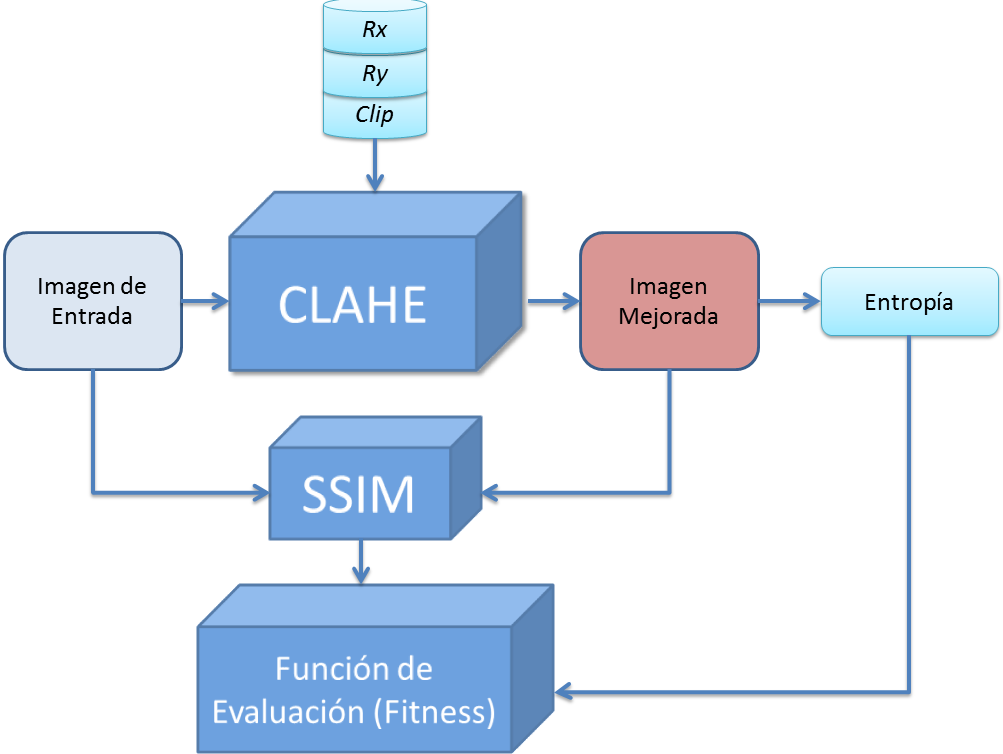
\includegraphics[width=8.5cm]{Figures/particula_clahe}}
  \vspace{0.5cm}
  \label{fig:particula_clahe}
  \captionof{figure}{Interacción entre CLAHE y SMPSO.}
\end{minipage}

\section{resultados y discusión}
\label{sec:resultadosdiscusion}

Se realizaron pruebas contra {\color{red} 7} imágenes de radiografía del tórax, de manera a comprobar la efectividad de la propuesta. En las Figuras \ref{fig:resultado1}, \ref{fig:resultado2} y \ref{fig:resultado3} se puede ver tanto la imagen original como el frente pareto conformado para los resultados obtenidos a partir de las ejecuciones de MPSO-CLAHE. En las Figuras {\color{red} FIGURAS RESULTANTES} se muestran algunos resultados que se encuentran en el frente pareto. En la tabla {\color{red}} se puede notar una relación inversa entre los objetivos, es decir al aumentar el coeficiente de entropía disminuye el SSIM; ésto es consistente con la premisa de que los objetivos son contradictorios. Se puede notar también según las apreciaciones hechas por una especialista, que en las radiografías del tórax se aprecian mejor los tejidos blandos al alcanzar determinado contraste (véase figuras {\color{red} PONER FIGURAS}) y a su vez las estructuras óseas se vuelven más visibles al alcanzar determinado contraste (véase Figuras {\color{red} PONER FIGURAS)}. En nuestra propuesta se obtiene una cantidad importante de imágenes resultantes con distintas relaciones de compromiso entre contraste y distorsión de manera automática, lo cual representa una ventaja porque se evita configurar los parámetros de mejora de forma arbitraria, como ocurre en \cite{1419470}.

\section{conclusiones}
\label{sec:conclusion}
Éste enfoque de mejora del contraste resulta sumamente interesante por los motivos expuestos en la sección anterior. Se están realizando más pruebas para validar los resultados, los cuales resultan muy prometedores. Se está trabajando también en encontrar otros tipos de imágenes a las que se puedan resaltar características de acuerdo al contraste aplicado, como efectivamente ocurre con las radiografías de tórax.



% Below is an example of how to insert images. Delete the ``\vspace'' line,
% uncomment the preceding line ``\centerline...'' and replace ``imageX.ps''
% with a suitable PostScript file name.
% -------------------------------------------------------------------------
%\begin{figure}[t]

%\begin{minipage}[b]{1.0\linewidth}
%  \centering
%  \centerline{
\includegraphics[width=8.5cm]{Figures/image1}}
%  \vspace{2.0cm}
%  \centerline{(a) Result 1}\medskip
%\end{minipage}
%
%\begin{minipage}[b]{.48\linewidth}
%  \centering
%  \centerline{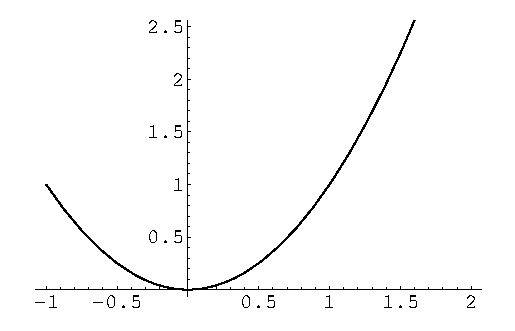
\includegraphics[width=4.0cm]{Figures/image3}}
%  \vspace{1.5cm}
%  \centerline{(b) Results 3}\medskip
%\end{minipage}
%\hfill
%\begin{minipage}[b]{0.48\linewidth}
%  \centering
%  \centerline{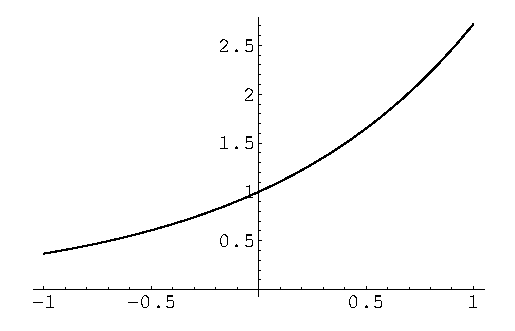
\includegraphics[width=4.0cm]{Figures/image4}}
%  \vspace{1.5cm}
%  \centerline{(c) Result 4}\medskip
%\end{minipage}
%
%\caption{Example of placing a figure with experimental results.}
%\label{fig:res}
%
%\end{figure}


% To start a new column (but not a new page) and help balance the last-page
% column length use \vfill\pagebreak.
% -------------------------------------------------------------------------
%\vfill
%\pagebreak

% References should be produced using the bibtex program from suitable
% BiBTeX files (here: refs). The IEEEbib.bst bibliography
% style file from IEEE produces unsorted bibliography list.
% -------------------------------------------------------------------------
\onecolumn
\noindent\begin{minipage}[b]{1.0\linewidth}
  \centering
   
   \begin{minipage}[b]{0.3\linewidth}  
   		\centering
   		\captionof{subfigure}{Resultados}
   		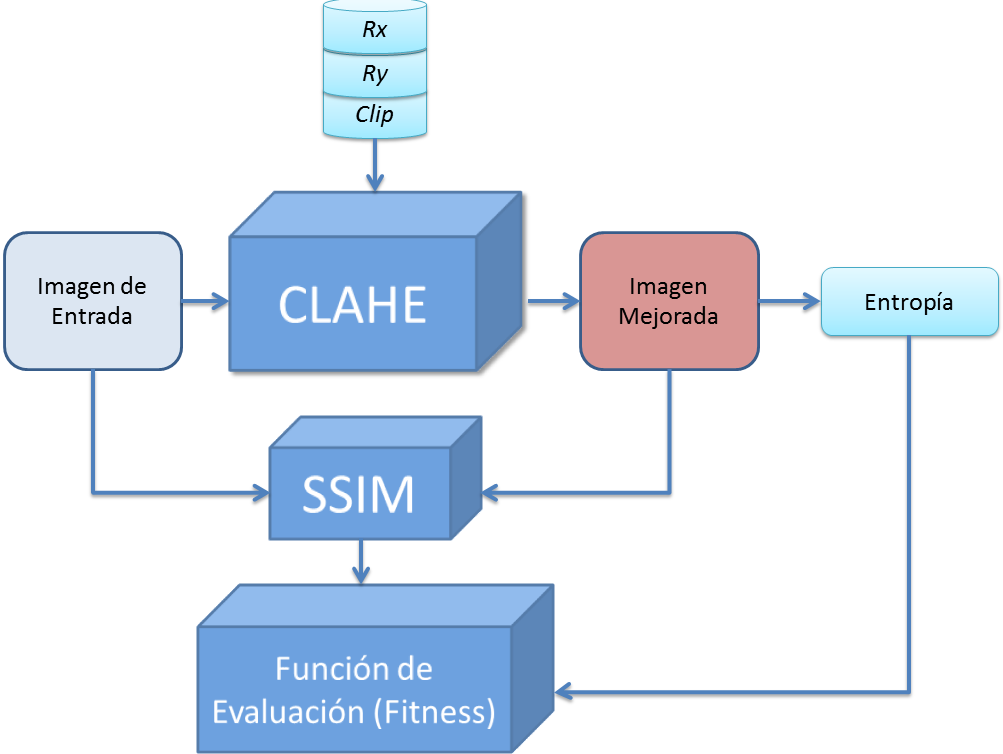
\includegraphics[width=2.5cm]{Figures/particula_clahe}
  	\end{minipage}
  \hspace{1pt}
   \begin{minipage}[b]{0.3\linewidth}  
   		\centering
   		\captionof{subfigure}{Resultados}
   		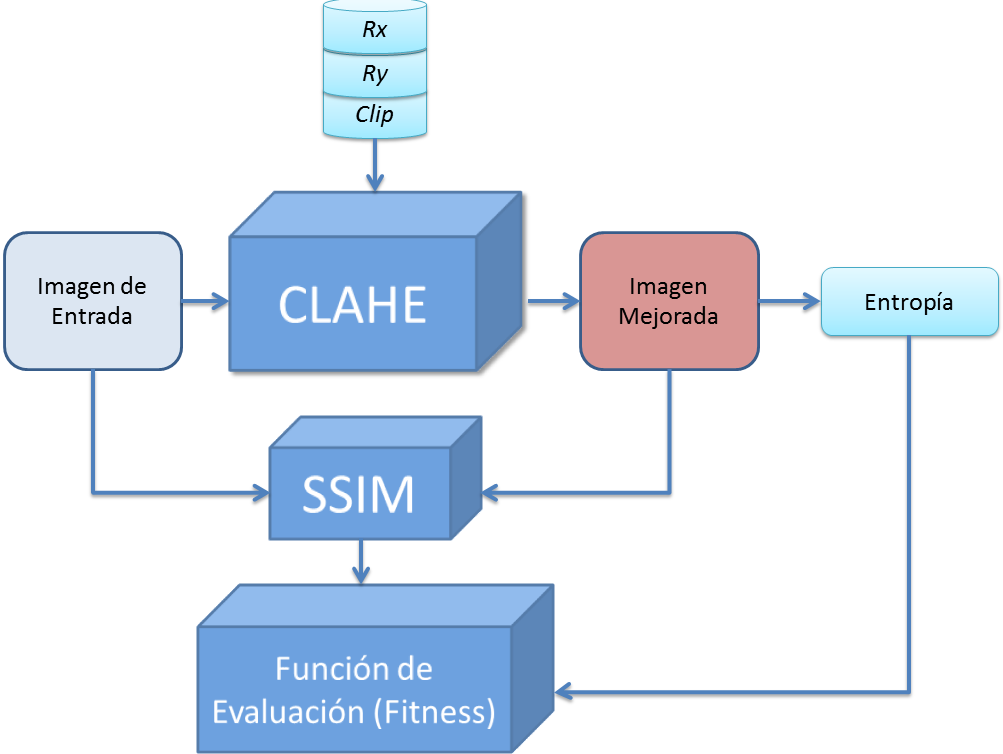
\includegraphics[width=2.5cm]{Figures/particula_clahe}
  	\end{minipage}
  \hspace{1pt}
   \begin{minipage}[b]{0.3\linewidth}  
   		\centering
   		\captionof{subfigure}{Resultados}
   		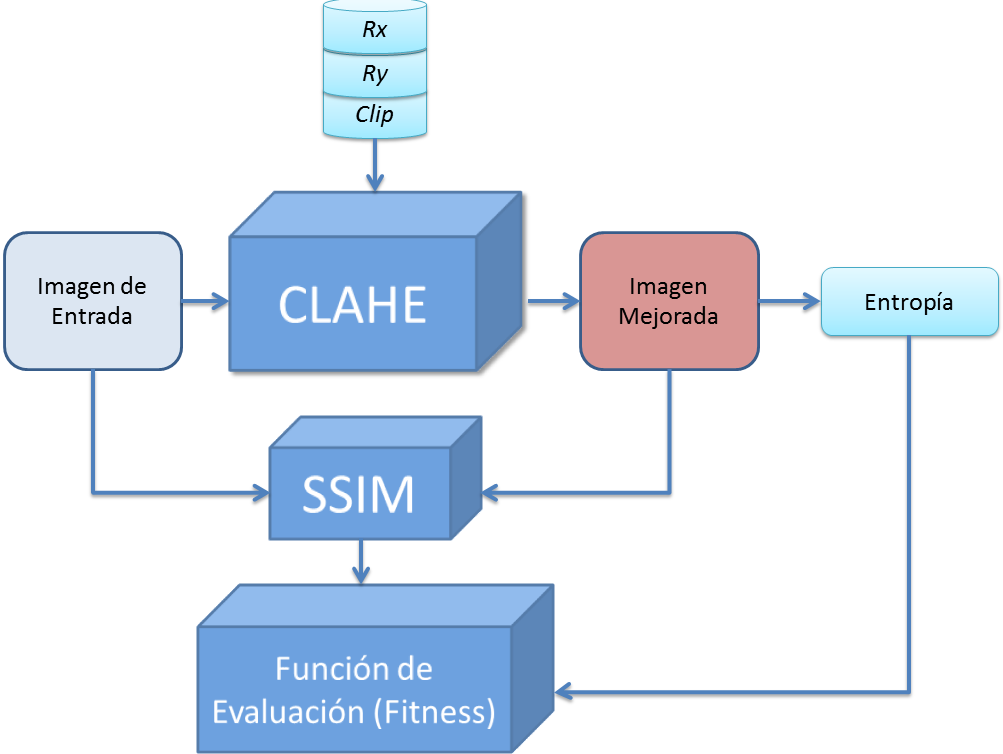
\includegraphics[width=2.5cm]{Figures/particula_clahe}
  	\end{minipage}
  \vspace{0.5cm}
    \label{fig:resultado1}
  \captionof{figure}{Resultados de PSO-CLAHE multiobjetivo. }

\end{minipage}

\begin{minipage}[b]{1.0\linewidth}
  
   \begin{minipage}[b]{0.3\linewidth}  
   		\centering
   		\captionof{subfigure}{Resultados}
   		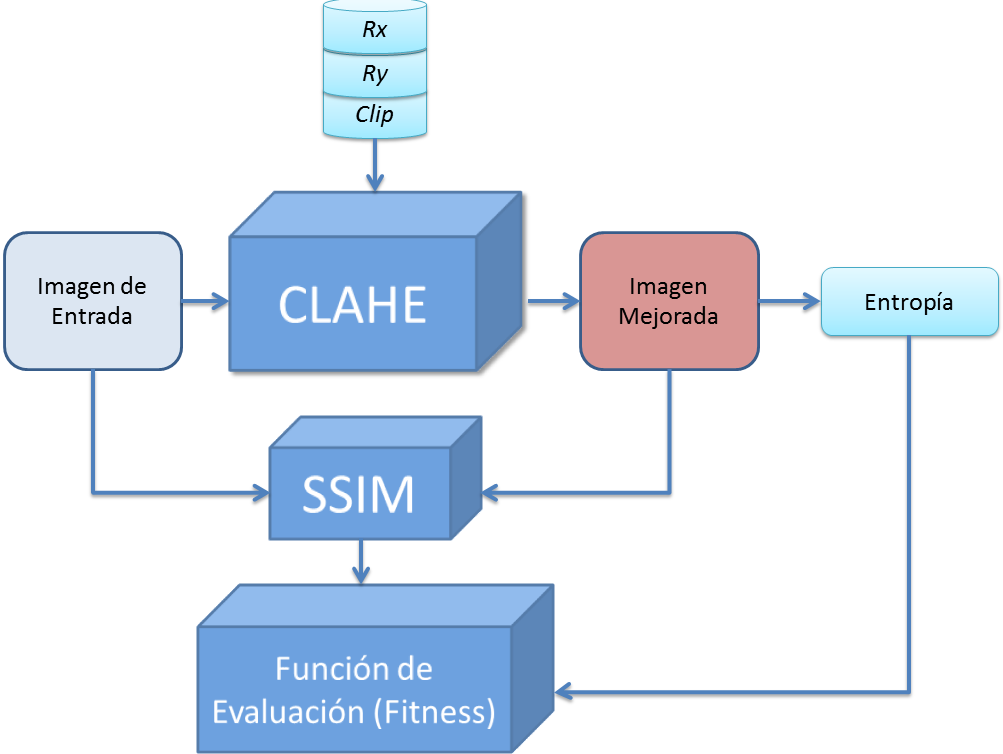
\includegraphics[width=2.5cm]{Figures/particula_clahe}
  	\end{minipage}
  \hspace{1pt}
   \begin{minipage}[b]{0.3\linewidth}  
   		\centering
   		\captionof{subfigure}{Resultados}
   		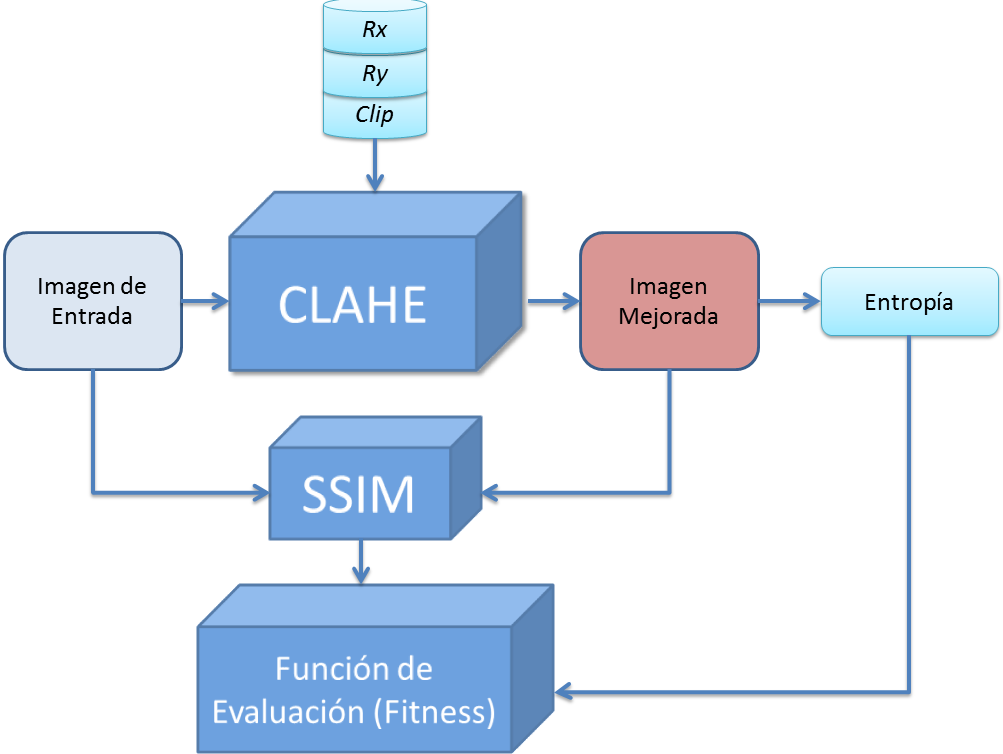
\includegraphics[width=2.5cm]{Figures/particula_clahe}
  	\end{minipage}
   \begin{minipage}[b]{0.3\linewidth}  
   		\centering
   		\captionof{subfigure}{Resultados}
   		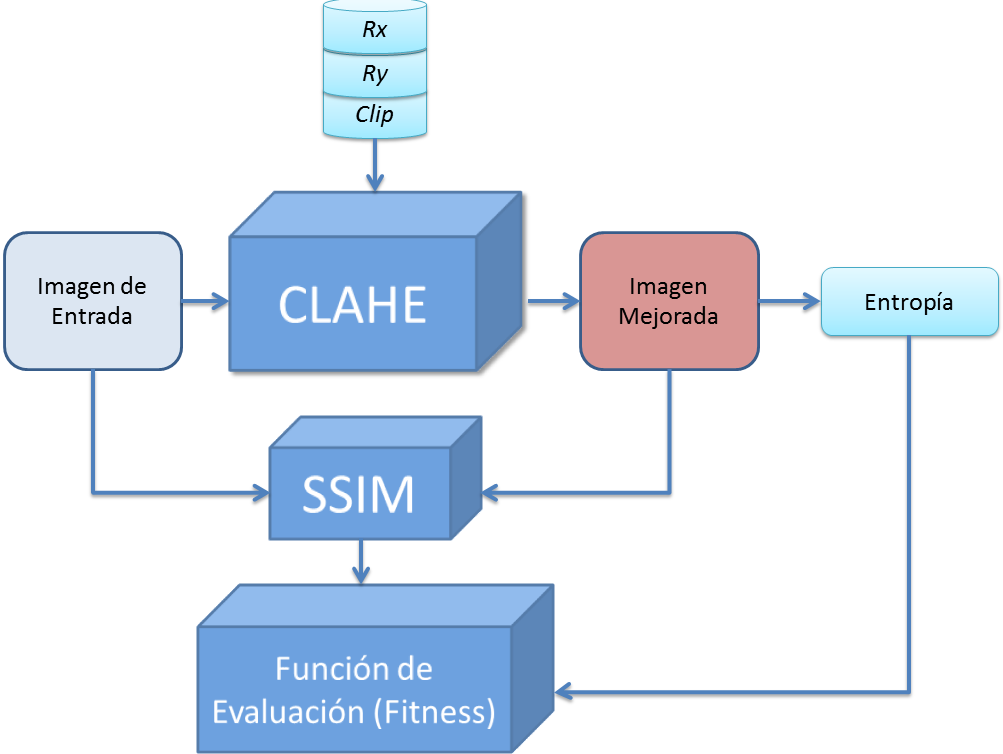
\includegraphics[width=2.5cm]{Figures/particula_clahe}
  	\end{minipage}
  \vspace{0.5cm}
    \label{fig:resultado2}
  \captionof{figure}{Resultados de PSO-CLAHE multiobjetivo. }

\end{minipage}

\begin{minipage}[b]{1.0\linewidth}
  \centering

   \begin{minipage}[b]{0.3\linewidth}  
   		\centering
   		\captionof{subfigure}{Resultados}
   		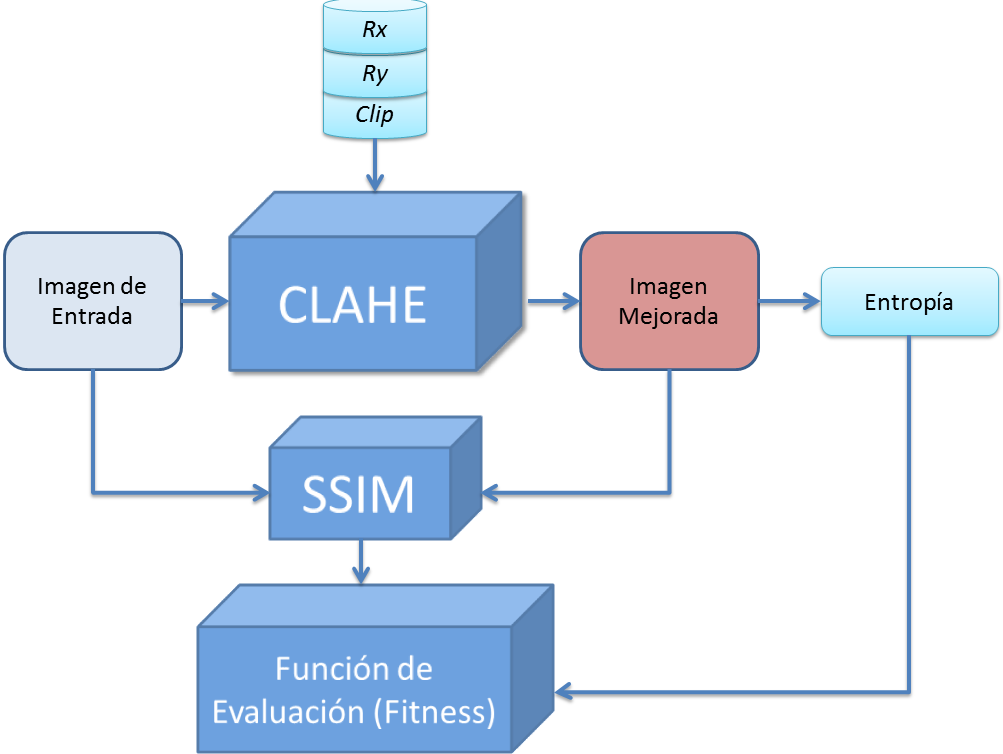
\includegraphics[width=2.5cm]{Figures/particula_clahe}
  	\end{minipage}
  \hspace{1pt}
   \begin{minipage}[b]{0.3\linewidth}  
   		\centering
   		\captionof{subfigure}{Resultados}
   		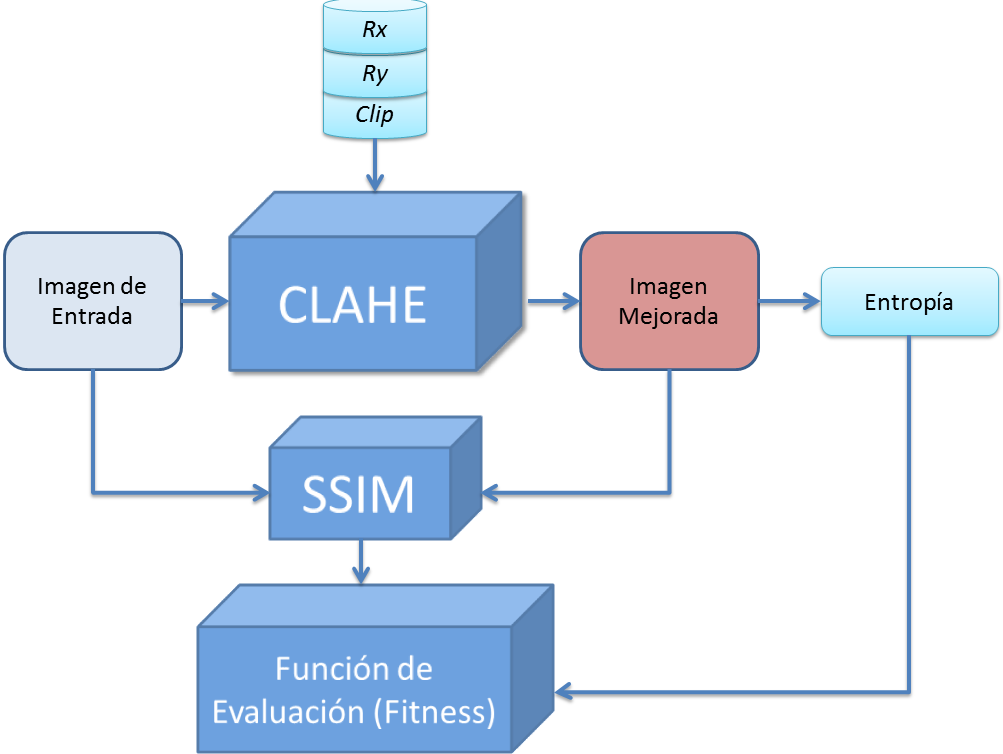
\includegraphics[width=2.5cm]{Figures/particula_clahe}
  	\end{minipage}
  \hspace{1pt}
   \begin{minipage}[b]{0.3\linewidth}  
   		\centering
   		\captionof{subfigure}{Resultados}
   		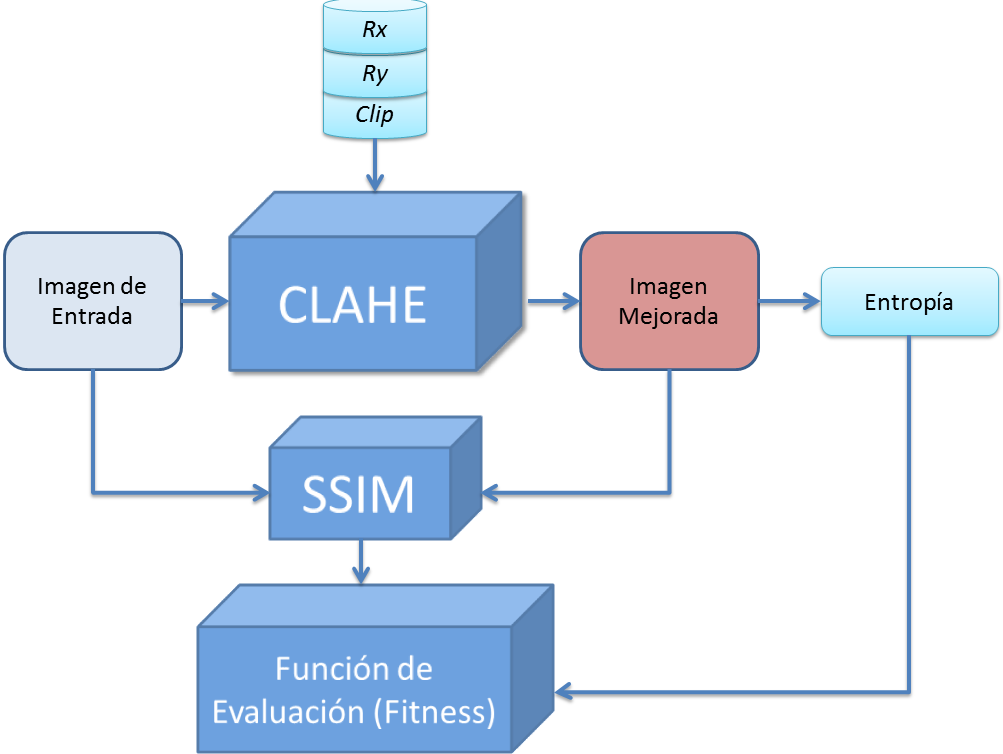
\includegraphics[width=2.5cm]{Figures/particula_clahe}
  	\end{minipage}
  \vspace{0.5cm}
    \label{fig:resultado3}
  \captionof{figure}{Resultados de PSO-CLAHE multiobjetivo. }

\end{minipage}


\twocolumn
\bibliographystyle{IEEEbib}
\bibliography{refs}



\end{document}
